\documentclass[fleqn,10pt,twoside]{gcb15submission}
\usepackage{url}\urlstyle{same}
\usepackage{booktabs}
\usepackage{colortbl, xcolor}

% rysunki
\usepackage{tikz}
\usepackage{ifthen}
\usepackage{xxcolor}
\usetikzlibrary{arrows}
\usetikzlibrary[topaths]
\usetikzlibrary{decorations.pathreplacing}

\title{signalHsmm - a novel semi-Markov model of eukaryotic signal peptides}

\author[1]{Micha\l{}  Burdukiewicz}
\author[2]{Piotr Sobczyk}
\author[1]{Pawe\l{} B\l{}a\.{z}ej}
\author[1]{Pawe\l{} Mackiewicz}
\affil[1]{University of Wroc\l{}aw, Department of Genomics, Poland}
\affil[2]{Wroc\l{}aw University of Technology, Department of Mathematics, Poland}

\keywords{signal petide prediction; n-gram; hidden semi-Markov models}

\begin{abstract}
The proper localization of proteins in a cell is essential to maintain their desired function. Information about the protein destination is included within the very protein in the form of short peptides called targeting signals. Ones of them are signal peptides, diverse N-terminal sequences, which are responsible for targeting of proteins to endomembrane system and their export outside the cell. Proteins equipped with signal peptides play crucial roles in metabolism, maintenance of tissue structure, immune response and regulation of other organismal functions. Moreover, the transport of proteins through the endomembrane system is important for their correct folding and posttranslational modifications. 

A common model of classical signal peptides assumes that they start with a positively charged n-region, followed by a hydrophobic h-region and a c-region ended with a cleavage site recognised by a signal peptidase. However, our studies of many protein sequences representing the wide range of diversified taxonomic organisms indicate a variability of signal peptides. Therefore, we designed a new, more univeral probabilistic model for eukaryotic signal peptides, which includes knowledge about their organisation, amino acid composition and variation.

The proposed model is based on hidden semi-Markov models (HSMMs) and use intrinsic knowledge about signal peptides. The big advantage of the algorithm is its extensibility. Using the n-grams (k-mers) we point how the general model can be attuned to yield not only better results, but also more information about signal peptides.

Our model was validated a signal peptide pedictor. It has showed the largest AUC=0.98 in comparison to other software and appeared very stable in the recovery of signal peptides after training even on very small data sets. Thanks to that, our model does not need to be permanently retrained with the continuous expansion of sequence databases. It should be emphasised that our model describes signal peptides from medically significant malaria parasites Plasmodium and their relatives (AUC = 0.92) more accurately than popular programs (0.84).

\end{abstract}

\begin{document}
\flushbottom
\maketitle
\thispagestyle{empty}


\section*{Introduction}

\subsection*{Signal peptides}

Proteins of eukaryotes are encoded in nuclear genomes and are synthetized in ribosomes located in the cytosol or bounded by the endoplasmic reticulum. After the translation process, proteins have to be targeted to specific subcellular compartments or exported outside the cell to the extracellular environment. The proper localization of proteins is essential to perform their desired function. Information about protein destination is included within the very protein in the form of short peptides or stretches of amino acid residues called targeting or sorting signals. Ones of them are signal peptides, which are located at the N-terminus of proteins.

Signal peptides are responsible for targeting of proteins via the Sec61 translocation channel~\citep{2007rapoportprotein} to endomembrane system, which includes endoplasmic reticulum, Golgi apparatus and endosomes. Such proteins can stay inside of these compartments, or can be inserted into cellular membranes or exported outside the cell. Proteins equipped with signal peptides constitute a substantial fraction of the whole proteome. They play crucial roles in metabolism ($\beta$ galactosidase, pepsins)~\citep{1991hofmannmutations}, maintenance of tissue structure (collagen)~\citep{2001chanaberrant}, immune response (interferons, interleukins)~\citep{2005zhangalteration} and regulation of other organismal functions (prolactin, glucagon)~\citep{2010huangrole}. Moreover, passing proteins through the endomembrane system is important for their correct folding and posttranslational modification such as glycosylation and phosphorylation.

Although signal peptides are quite variable, some general architecture were proposed~\citep{1994izardsignal, 2013vossmechanism} - Fig. \ref{fig:sparch}. It is assumed that signal peptides start with a positively charged sequence of amino acid residues, called the n-region with the length of about 5-8 residues. They probably enforce a proper topology on the polypeptide during translocation through membrane based on the positive-inside rule~\citep{1988vonheijnetopogenic}. The first region is followed by a stretch of hydrophobic amino acids (h-region) with the length of about 8-12 residues. It constitutes a core region of signal peptide and has a tendency to form $\alpha$-helix. The third part of a signal peptide, usually 6 residues long, is a polar, but uncharged c-region ended with a cleavage site recognized by the signal peptidase. The amino acid composition and the length of these regions vary between signal peptides, which influences the efficiency of protein secretion~\citep{2006hegdethe}.

\begin{figure}[ht]\centering
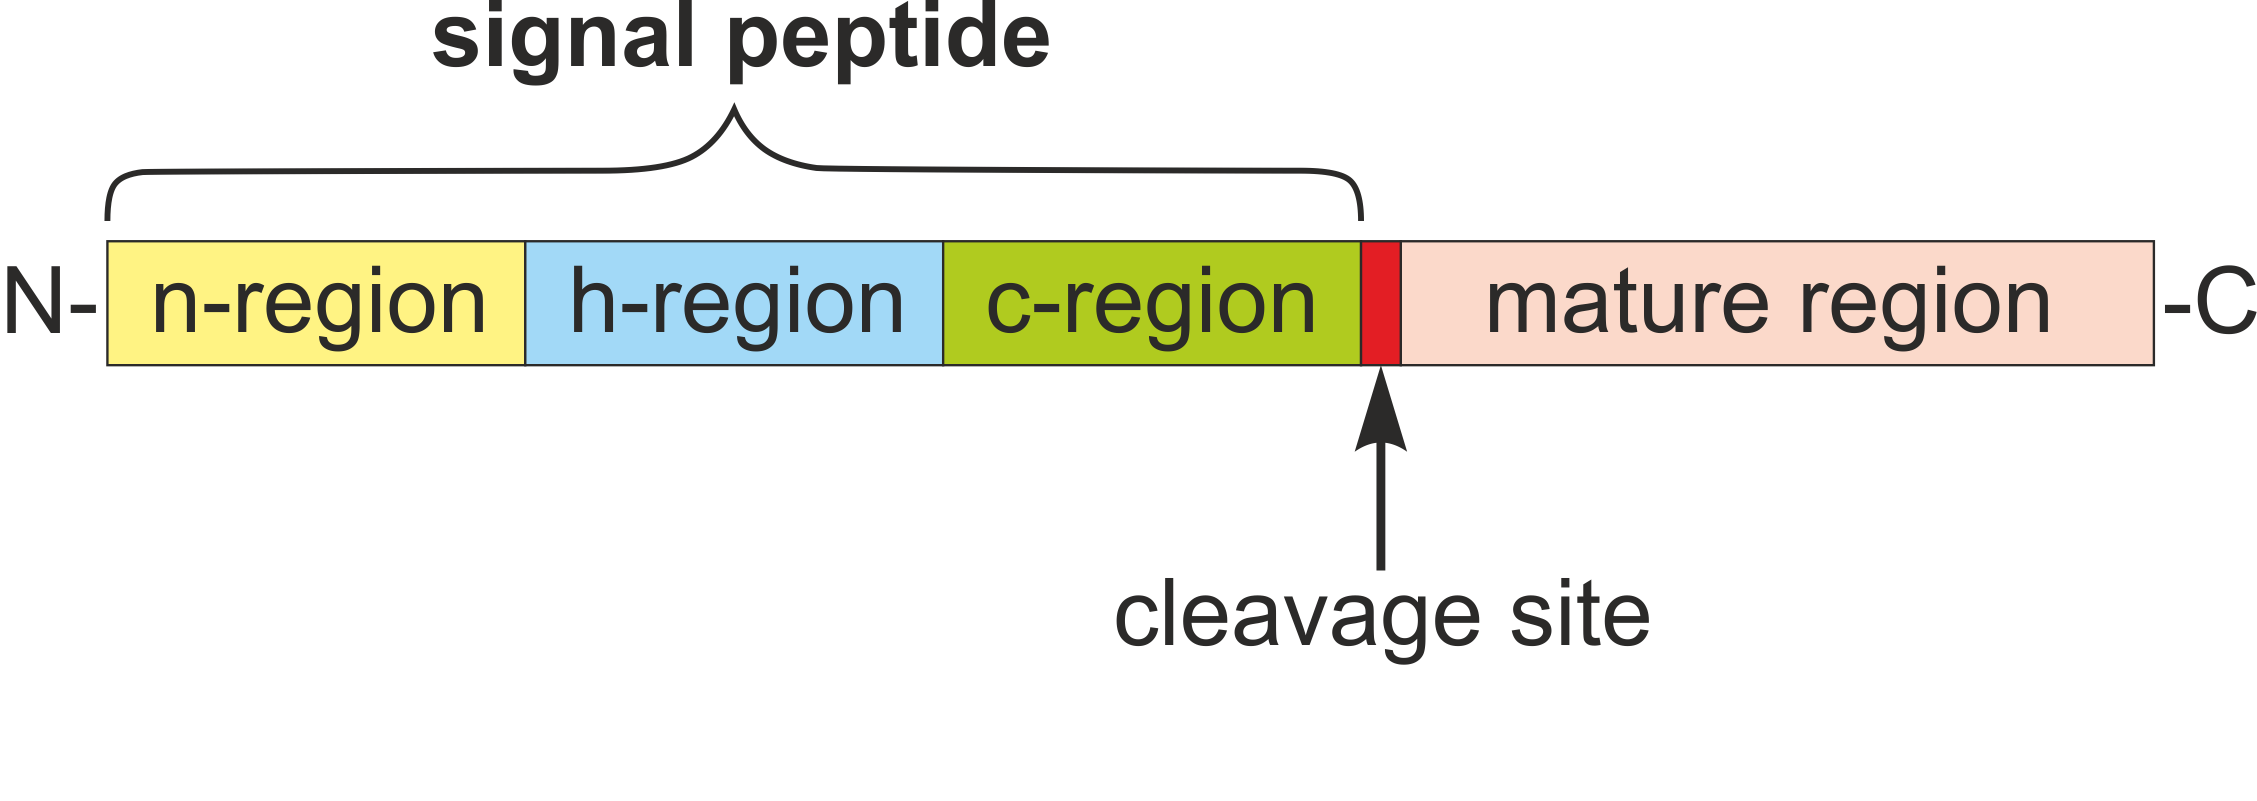
\includegraphics[width=0.55\textwidth]{figures/SP.png}
\caption{The organization of signal peptide.}
\label{fig:sparch}
\end{figure}

During or after translocation of the protein into the lumen of endoplasmic reticulum, the typical signal peptide is cleaved by a signal peptidase~\citep{2002paetzelsignal} and next degraded by specific proteases, whereas the rest (mature) part of protein stays in the lumen or is passed to other compartments. The cleavage site is characterized by a very variable amino acid composition. It typically contains small and neutral residues at -3 and -1 positions~\citep{1994palzkillselection}. The site is, however, absent from some membrane proteins in which the first transmembrane-domain acts both as signal peptides and signal anchor~\citep{1988szczesnaskorupapositive}.

Some data indicate that signal peptides may be universal. It was found, for example, that even bacterial signal peptides targeted correctly transgenic proteins to the plant~\citep{2009moellera} or mammalian secretory system~\citep{2014naganoestablishment}. On the other hand, signal peptides show great variation and the description presented above (Fig. \ref{fig:sparch}) refers to the most ‘typical’ signal peptides. There are also exceptionally long signal peptides, which fulfil more sophisticated roles~\citep{2009hissarchitecture}. For example, the fragment of signal peptide from preprolactin probably takes part in the regulation of prolactin secretion. Other examples are signal peptides of MHC class I, which inhibit activity of NK cells. Interesting functions have signal peptides of viral origin, which are involved in the immune evasion or viral life cycle~\citep{2000kappposttargeting}. Such diverse functions are restricted not only to the long signal peptides. The peptides from midkine, a protein contributing to the tumor progression, contains epitopes recognized by CD4+ T cells~\citep{2013kerzerhothe}. It indicates that the signal peptide may participate in a tumor immunity. The functional significance of these targeting signals makes that the prediction of signal peptide-containing proteins is also an important step in the drug development~\citep{2005zhangalteration, 2012netoadeimproving, 2010moellerwetmilling}.


\subsection*{Signal peptide predicting software}

Although many experimental methods determining the subcellular localization of proteins were devised, they are time consuming and laborious. Therefore, the development of new approaches in the field of computational biology and bioinformatics is desirable. They are not only a good support, complement or alternative for the experimental methods but also enable to understand rules encoding information about protein targeting, which is contained in the predicted targeting signals. However, many of the present predictors disregard full biological information carrying by signal peptides.

Having functional importance and specific features, signal peptides became the subject of many programs to their prediction based on different methods. The state of the art software for predicting the presence of signal peptides often incorporates ‘black-box’ models, as neural networks~\citep{2011petersensignalp}, support vector machines~\citep{2014zhangprediction}, Bayesian networks~\citep{2012zhengsignalbnf} or k-nearest neighbours~\citep{2007shensignall}. Such models neither utilize biological information about signal peptides nor work properly on atypical signal peptides. 

The other type of software incorporates into the prediction process theoretical knowledge about the structure of signal peptides. Although these programs do not share innate flaws of ‘black-box’ models, they also demand an improvement. Some of them are based on position matrices or their more abstract variants~\citep{2014zhangprediction, 2004hillerpredisi}. Others (Phobius, Philius and not supported SignalP 3.0) use hidden Markov models (HMMs)~\citep{2004klla, 2008reynoldstransmembrane, 2004bendtsenimproved}, which reflect regions of signal peptides without realizing limitations of this probabilistic framework. However, the HMMs imply geometric distribution for duration of region length. We replicated the rules for extracting regions' boundaries from the first work utilizing HMMs in prediction of signal peptides~\citep{1998nielsenprediction} and found that the mentioned assumption is not in concordance with the reality because every region revealed the length distribution other than geometric (Fig. \ref{fig:reglen}). Moreover, the commonly used rigid region scheme (Fig. \ref{fig:sparch}) does not describe extremely long or short signal peptides. Theoretically, HMMs that describe the atypical signal peptides could be developed to consider also unusual structures, but such probabilistic frameworks have not still been implemented.

\begin{figure}[ht]\centering
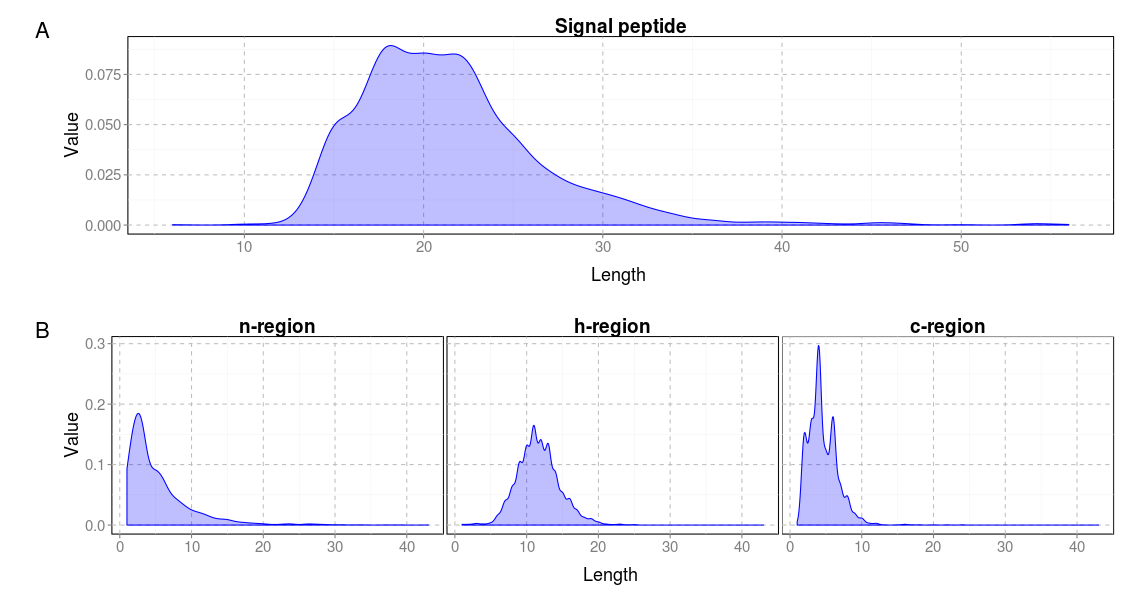
\includegraphics[width=0.9\textwidth]{figures/reglen.png}
\caption{A) Distribution of lengths of signal peptides. B) Distribution of the lengths of signal peptide regions. The measure of the length is a number of amino acids in the subsequence. The data was extracted from 2~589 signal peptide sequences derived from UniProt database (see \textbf{Data selection} in \textbf{Methods}).}
\label{fig:reglen}
\end{figure}


Another feature, shared by majority of the signal peptide predicting software, is the orthogonal encoding of amino acids, in which a vector of 20 digits represents every amino acid. This method of encoding, however, does not preserve relationships between amino acids. The distance between residues is the same regardless of the similarity of their physicochemical properties. Such behaviour is especially undesired in signal peptides models because their regions are defined by specific features of amino acid residues and not by the simple occurrence of specific amino acids. In addition to this, such sparse encoding enforces larger data sets, which hinders their management and analysis~\citep{2002linamino}.

All programs used in signal peptide recognition are trained on real protein sequences. Therefore, they succeed in the recognition of peptides similar to those in the learning set, but fail in the case of artificial signal peptides. Such peptides are designed to increase effectiveness of protein secretion~\citep{2010futatsumorisugaisignal}. They are especially important in industrial applications to increase yield of proteins. Therefore, only explicit knowledge about the organization of signal peptides allows creating sequences that will be the most efficient in the export of proteins~\citep{2013ngengineering}. Signal peptides have also an important application in gene therapy. Mimicking the natural mechanism of protein export, artificial signal peptides with tumor epitopes increase the antitumor immune response~\citep{2003heenhanced}. Such epitopes must be properly inserted into a signal peptide without decreasing its secretion properties through disruption of the regional structure. Instead of time-consuming and expensive laboratory experiments, it would be very useful to survey in silico many artificial peptides to select the ones that would fulfil the designed role.


\section*{Methods}

\subsection*{Overview}

The functionality of a signal peptide depends not on exact sequence of specific amino acids, but on the physicochemical properties of residues in a given region. Henceforth, the usage of raw amino acid sequences is superfluous and introduces unnecessary information. To utilize this property of signal peptide recognition, we cluster amino acids into several groups based on the physicochemical properties of residues.

The pre-processed sequences are further analyzed by the heuristic algorithm, which determines borders between three characteristic signal peptide regions, the enhanced version of algorithm presented in~\cite{1998nielsenprediction}. Using the current information from experimentalists, we refined the region recognition criteria.

Next, two models are trained to recognize proteins with and without a signal peptide. The first one is a hidden semi-Markov model, in which each of three signal peptide regions is represented by a different hidden state. The additional fourth hidden state represents mature protein. Each state is described by the frequencies of amino acid groups  within that state. The distribution of hidden states durations, the number of amino acids related to each hidden state in signal peptide, is based on the empirical density of region lengths from the training set. 

The second model is a simple probabilistic approach in which no association between amino acids was assumed, and probability of amino acids groups occurrence was determined by their frequencies in mature proteins.

\subsection*{Data selection}


Eukaryotic protein sequences and their annotations were properly prepared according to the literature of the subject and downloaded from UniProt database release 2015\_06. The positive set contained 2~589 sequences with an experimentally confirmed signal peptide and its cleavage site. Sequences with more than one cleavage site were excluded from the final data set. The negative set comprised 152~272 sequences without any signal peptide annotation. Protein sequences with ambiguous symbols: X, J, Z and B were removed from the final sets. Proteins with selenocysteine (U) were also excluded from data set, because there are no records of signal peptides containing this amino acid.

\subsection*{Clustering of amino acids}

Amino acids were clustered using several criteria relevant for the architecture of signal peptide: hydrophobicity, frequency in alpha-helices, polarity and size. High hydrophobicity is a determinant of the h-region, the core of signal peptides. Alpha-helix, the secondary structure of the h-region, is probably induced by the positively charged n-region. High polarity as well as smaller size are important features of the residues in the cleavage site~\citep{1994palzkillselection}.

\begin{table}[ht]
\centering
\begin{tabular}{ll}
  \toprule
Criterion name & Property name \\ 
  \midrule
Size & Size \\ 
   \rowcolor[gray]{0.85}Size & Molecular weight \\ 
  Size & Residue volume~\citep{1973goldsackcontribution} \\ 
   \rowcolor[gray]{0.85}Size & Bulkiness~\citep{1968zimmermanthe} \\ 
  Hydrophobicity & Normalized hydrophobicity scales for alpha-proteins~\citep{1992cidhydrophobicity} \\ 
   \rowcolor[gray]{0.85}Hydrophobicity & Consensus normalized hydrophobicity scale~\citep{1984eisenbergthreedimensional} \\ 
  Hydrophobicity & Hydropathy index~\citep{1982kytea} \\ 
   \rowcolor[gray]{0.85}Hydrophobicity & Surrounding hydrophobicity in alpha-helix~\citep{1980ponnuswamyhydrophobic} \\ 
  Polarity & Polarity~\citep{1974granthamamino} \\ 
   \rowcolor[gray]{0.85}Polarity & Mean polarity~\citep{1988radzickainfluences} \\ 
  Frequency in alpha-helices & Signal sequence helical potential~\citep{1982argosstructural} \\ 
   \rowcolor[gray]{0.85}Frequency in alpha-helices & Normalized frequency of N-terminal helix \\ 
  Frequency in alpha-helices & Relative frequency in alpha-helix~\citep{1990prabhakaranthe} \\ 
   \bottomrule
\end{tabular}
\caption{Properties used in clusterization.} 
\label{tab:aaprop}
\end{table}

We selected 13 properties from AAIndex database~\citep{2008kawashimaaaindex} (see Table~\ref{tab:aaprop}), each attributed to a single criterion. We established 96 permutations of the properties, where each permutation contains only one property associated with a given criterion. Considering all permutations of properties, we created 96 possible clusterings of amino acids using Euclidean distance and Ward's method. Further, we cut the clusterings to create four-group encodings. As expected, some encodings (31\%) were identical.

To compare encodings we performed a 5-fold cross-validation training a new instance of signalHsmm on every encoding. We created balanced data sets by subsampling a number of proteins without a signal peptide equal to the number of proteins with signal peptide.
The analysis was carried using also redundant encodings, but results are not shown (HSMM is a deterministic algorithm and predictions for identical groupings of amino acids were the same). The cross-validation was repeated XXX times, to ensure that every negative protein was tested at least once with XXX probability.

\subsection*{Hidden semi-Markov model}
Hidden semi-Markov model (HSMM) is an extension of hidden Markov model (HMM).
As such, it proved to yield better performance in many fields of bioinformatics including
gene recognition~\citep{Pachter02applicationsof}, protein secondary structure prediction~\citep{16571137}
or automatic detection of heartbeats~\citep{7043102}.
Let us first briefly describe the idea that lies behind HMM. 
Suppose you have a sequence of observations e.g. amino acids, and you are interested in understanding underlying cause of their occurrence. 
HMM aims to answer that question by assuming a specific, yet flexible, structure of the problem.
HMM consists of two stochastic processes. First is discrete Markov chain $X_{t=1}^T$ on the set of so called hidden states $\{S_1, \dots S_n\}$.
They are "the cause" of the observations. At every step $t$, hidden state might change according to transition matrix
$A= (a)_{i,j=1}^n$, where $a_{i,j} = \mathcal{P}(X_{t+1} = S_j | X_t = S_i)$. In our application hidden states are signal peptide regions.
Second process $E_{t=1}^T$ is observation process, defined on the set of possible observations $\{O_1, \dots, O_m\}$. 
Observations are assumed to occur independently. Their distribution depends only on hidden state which emits it. 
Probabilities are given by a matrix $B$, $b_{i,k} = \mathcal{P}(E_t = O_k | X_t = S_i)$.
In our case, observations are (degenerated) amino acids.
Main goal in signalHsmm is to find, for a given peptide, most probable regions boundaries. This is achieved with
Viterbi algorithm.
For a good reference on HMM see~\citep{1989rabinera}.

In regular HMM, hidden state duration -- number of observations emitted by the hidden state, has geometric distribution.
\citep{Durbin98biologicalsequence} shows how to extend it for some different distributions without significant increase in computational 
complexity. Similar ideas were used for signal peptide recognition, for example in~\citep{2004klla}. 
It is, however, still not flexible enough. Empirical regional length distributions (see figure~\ref{fig:reglen})
are difficult to capture in that way.

%rysunek pokazujący o co chodzi w HMM
\begin{figure}[h]
\centering
\tikzstyle{block} = [draw,shape=circle, top color=white, bottom color=green!50!red!70 ,minimum size=4em]
\tikzstyle{blockComp} = [draw,shape=circle, top color=white, bottom color=red!50!black!70 ,minimum size=2.5em]
% diameter of semicircle used to indicate that two lines are not connected
\def\radius{.7mm} 
\tikzstyle{branch}=[shape=rectangle, top color=white, bottom color=green!50!red!70 ,minimum size=3pt,inner sep=0pt]
\tikzstyle{branch2}=[shape=rectangle, top color=white, bottom color=red!50!black!70 ,minimum size=3pt,inner sep=0pt]
\def\n{11}
 \tikzstyle{line} = [draw=black, color=black!30!white!50, line width=1.5mm, -latex'] 
 \tikzstyle{line2} = [draw=black, color=red!30!black!50, line width=1.5mm, -latex']
\tikzstyle{frame}=[text=black,above, bottom color=white, top color=blue!50!black!70  ]
\tikzstyle{frameComp}=[text=black,below, bottom color=white, top color=red!50!black!70  ]
 \tikzstyle{line3} = [color=green!50!red!70, line width=1.5mm]
\def\names{{"$O_{1,1}$","...","$O_{1,d_1}$", "...","$O_{k, 1}$", "...", "$O_{k, d_k}$"}}%
\begin{tikzpicture}[>=latex']
%wąsate nawiasy
\draw [decorate, decoration={brace,amplitude=10pt},line3,xshift=0pt,yshift=0pt] (2.5,1) -> (10.5,1) node [branch,midway,yshift=0.8cm,color=black] 
	{\textbf{Hidden states}};
% \draw [->,decoration={brace,mirror,amplitude=10pt},line2,xshift=0pt,yshift=0pt] (11,-3) -- (3,-3) node [branch2,midway,yshift=-0.6cm,color=black] 
% 	{\textbf{Kierunek odczytu na nici Cricka ($3' \to 5'$)}}; 
   % Draw blocks, inputs and outputs
 
\node[block, text width=3em] at (1+2,0) (block1) {\footnotesize 1st hidden state};
\node[blockComp] at (-.5+2,-2)  (komp1) {\footnotesize \pgfmathparse{\names[0]}\pgfmathresult};
\node[blockComp] at (1+2,-2)  (komp2) {\footnotesize \pgfmathparse{\names[1]}\pgfmathresult};
\node[blockComp] at (2.5+2,-2)  (komp3) {\footnotesize \pgfmathparse{\names[2]}\pgfmathresult};
\draw[line,->]  (block1) --  (komp1);
\draw[line,->]  (block1) --  (komp2);
\draw[line,->]  (block1) --  (komp3);
\draw[line3,->] (block1.east) -- +(2,0) node [branch,midway,yshift=0.2cm,xshift=-0.2cm,color=black] {\footnotesize \textbf{transition}};

\node[block, bottom color=green!50!red!80,] at (4.5+2,0) (block2) {...};
\draw[line3,->] (block2.east) -- +(2,0) node [branch,midway,yshift=0.2cm,xshift=-0.2cm,color=black] {\footnotesize \textbf{transition}};
\node[blockComp] at (4.5+2,-2)  (komp4) {\footnotesize \pgfmathparse{\names[3]}\pgfmathresult};
\draw[line,->]  (block2) --  (komp4) ;

\node[block,text width=3em, bottom color=green!50!red!90] at (8+2,0) (block3) {\footnotesize $k^{th}$ hidden state};
\node[blockComp] at (6.5+2,-2)  (komp5) {\footnotesize \pgfmathparse{\names[4]}\pgfmathresult};
\node[blockComp] at (8+2,-2)  (komp6) {\footnotesize \pgfmathparse{\names[5]}\pgfmathresult};
\node[blockComp] at (9.5+2,-2)  (komp7) {\footnotesize \pgfmathparse{\names[6]}\pgfmathresult};
\draw[line,->]  (block3) --  (komp5);
\draw[line,->]  (block3) --  (komp6);
\draw[line,->]  (block3) --  (komp7);

% \draw[<->, color=red!30!black!50, line width=1.5mm] (komp1) |- +(5,-1.5) node[line2, yshift=-0.5cm] {\textbf{Observations}} -| (komp7); 

\draw [color=red!30!black!50, line width=1.5mm, decorate,decoration={brace,amplitude=10pt,mirror,raise=10pt},yshift=-10pt]
(1,-1.8) -- (5,-1.8) node [branch2, midway, yshift=-1cm,color=black] {\textbf{Duration of length $d_1$}};

\draw [color=red!30!black!50, line width=1.5mm, decorate,decoration={brace,amplitude=10pt,mirror,raise=10pt},yshift=-10pt]
(8,-1.8) -- (12,-1.8) node [branch2, midway, yshift=-1cm,color=black] {\textbf{Duration of length $d_k$}};

\draw [color=red!30!black!50, line width=1.5mm, decorate,decoration={brace,amplitude=20pt,mirror,raise=10pt},yshift=-10pt]
(1,-2.8) -- (12,-2.8) node [branch2, midway, yshift=-1.5cm,color=black] {\textbf{Observations, $\sum_{i=1}^k d_i = T$}};

\end{tikzpicture}
\caption{General scheme of hidden semi-Markov model}
\label{fig:hsmm}
\end{figure}

The model we use is Hidden semi-Markov Model(HSMM)~\citep{Yu2010215}. It extends HMM by allowing 
any given hidden state duration distribution. Diagram of HSMM is presented in figure~\ref{fig:hsmm}.
In addition to matrices $A$ and $B$, model is given by probabilities of duration length in hidden states.
$$\mathcal{P}(\text{duration in state} = d | \text{state is } S_i), \;\; i = 1, \dots, n, \;\; d = 1, \dots, D$$
where $D$ is maximum allowed duration.
As our datasets are of reasonable size, $D$ is small -- around 30, computational effort is not much 
higher than with the regular HMM. 

The model we use has a very specific structure. Hidden states are signal peptide regions.
Almost all entries in transition matrix $A$ are zeros, because regions are sequential.
Possible transitions are depicted as arrows in figure~\ref{fig:signalHsmm}.
Probabilities of observations for hidden states and hidden states durations were estimated from training data.
The advantage of HSMM model is not only a better performance but also its straightforwardness.
Figure~\ref{fig:signalHsmm} is easy to interpret for a researcher without any mathematical background.

%model structure
\begin{figure}
 \begin{minipage}{.5\linewidth} 
     \resizebox{6.5cm}{!}{%
    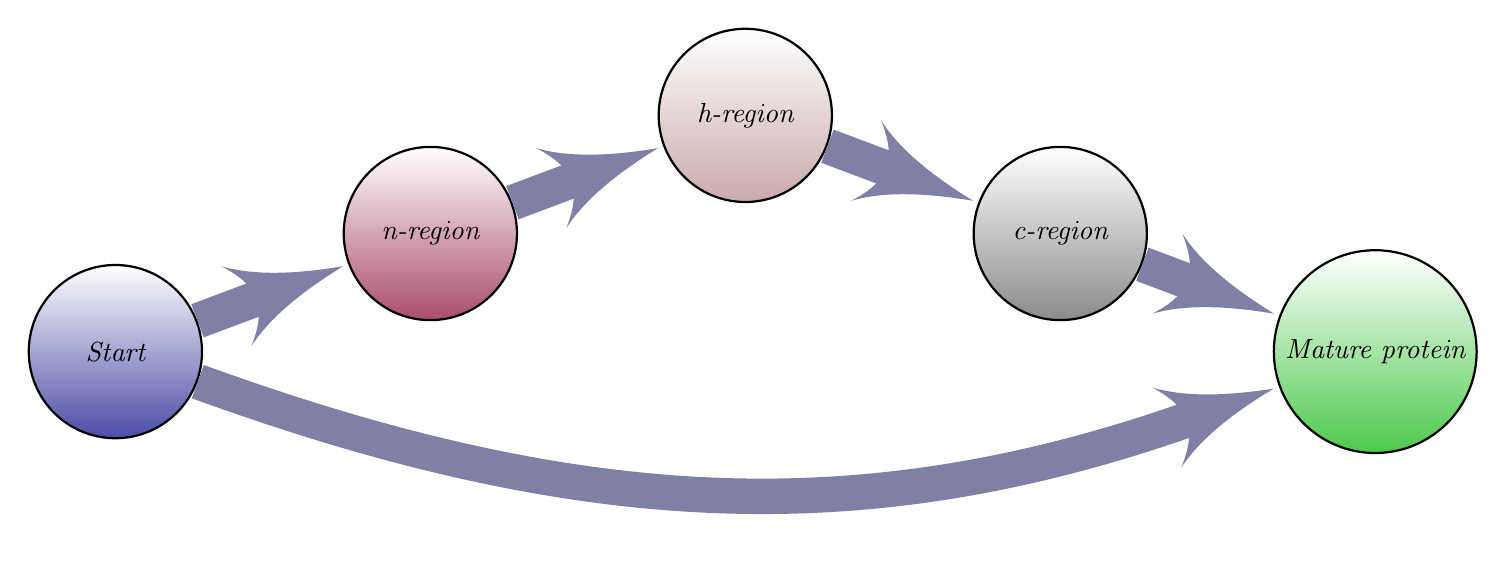
\begin{tikzpicture}[->,>=stealth',shorten >=2pt,auto,node distance=4.5cm, thick]
    \label{fig:model_hsmm}
      \tikzstyle{line} = [draw=black, color=blue!30!black!50, line width=4.5mm, -latex']
      \tikzstyle{main node} = [circle,fill=blue!20,draw, minimum size = 2.2cm, font=\itshape,
         align=center,  top color=white, bottom color=blue!50!black!70 ] %font=\sffamily\small\bfseries,
      %nodes
      \node[main node]            (start') 	[]						{Start};	     
      \node[main node, bottom color=purple!70!black!70] 	(nregion') 	[right of=start',xshift=-5mm, yshift=15mm] 	{n-region};
      \node[main node, bottom color=pink!70!black!70] 	(hregion') 	[right of=nregion',xshift=-5mm,yshift=15mm] 	{h-region};
      \node[main node, bottom color=gray!70!black!70] 	(cregion') 	[right of=hregion',xshift=-5mm,yshift=-15mm] 	{c-region};
      \node[main node, bottom color=green!70!black!70] 	(mature') 	[right of=cregion',xshift=-5mm, yshift=-15mm] 	{Mature protein};
      
      %lines
      \path [line] (start')   edge node [left, color=black] {} (nregion');
      \path [line] (nregion') edge node [below, color=black] { } (hregion');
      \path [line] (hregion') edge node [below, color=black] { } (cregion');
      \path [line] (cregion') edge node [left, color=black] { } (mature');
      \draw [line] (start') to[out=340,in=200] (mature');
    \end{tikzpicture} }
    \caption{The diagram of signalHsmm.}
    \label{fig:signalHsmm}
\end{minipage}
 \begin{minipage}{.5\linewidth}
     \resizebox{6.5cm}{!}{%
    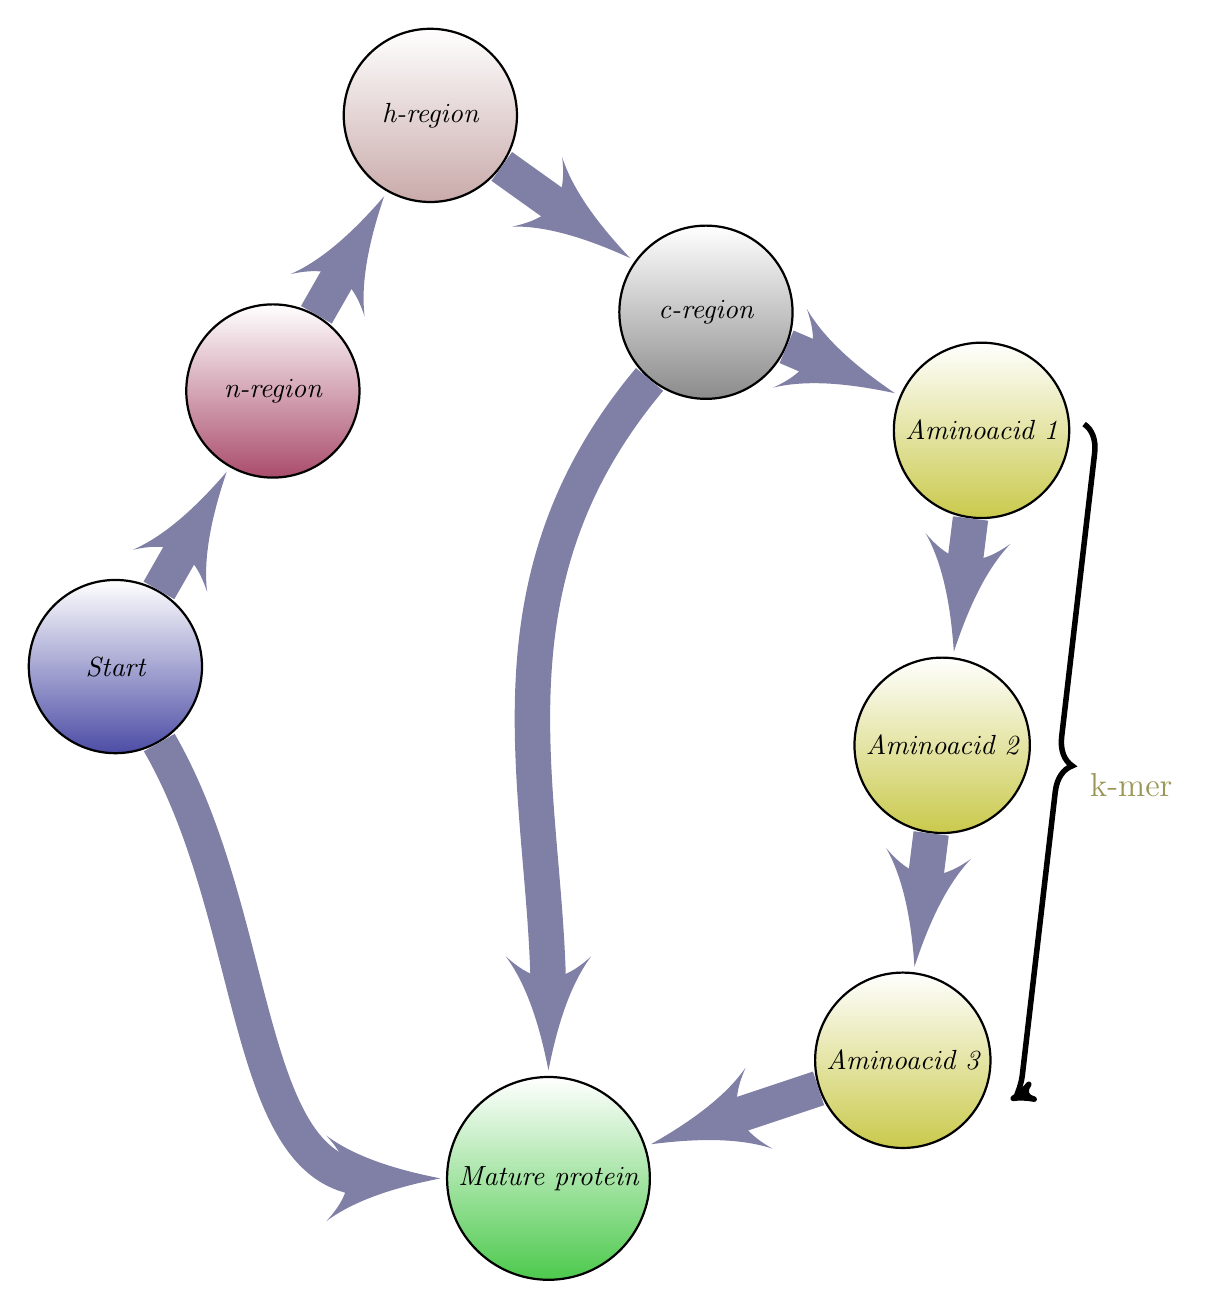
\begin{tikzpicture}[->,>=stealth',shorten >=2pt,auto,node distance=4.5cm, thick]
    \label{fig:model_hsmm_kMer}
      \tikzstyle{line} = [draw=black, color=blue!30!black!50, line width=4.5mm, -latex']
      \tikzstyle{main node} = [circle,fill=blue!20,draw, minimum size = 2.2cm, font=\itshape,
         align=center,  top color=white, bottom color=blue!50!black!70 ] %font=\sffamily\small\bfseries,
      %nodes
      \node[main node]            (start')   []  					{Start};	     
      \node[main node, bottom color=purple!70!black!70] 	(nregion') 	[right of=start',xshift=-25mm, yshift=35mm] 	{n-region};
      \node[main node, bottom color=pink!70!black!70] 	(hregion') 	[right of=nregion',xshift=-25mm,yshift=35mm] 	{h-region};
      \node[main node, bottom color=gray!70!black!70] 	(cregion') 	[right of=hregion',xshift=-10mm,yshift=-25mm] 	{c-region};
      \node[main node, bottom color=green!70!black!70] 	(mature') 	[below of=hregion',xshift=15mm, yshift=-90mm] 	{Mature protein};
      
      \node[main node, bottom color=yellow!70!black!70]   (kmer1) 	[below of=cregion',xshift=35mm,yshift=30mm] 	{Aminoacid 1};
      \node[main node, bottom color=yellow!70!black!70]   (kmer2) 	[below of=kmer1,xshift=-5mm,yshift=5mm] 	{Aminoacid 2};
      \node[main node, bottom color=yellow!70!black!70]   (kmer3) 	[below of=kmer2,xshift=-5mm,yshift=5mm] 	{Aminoacid 3};
      %lines
      \path [line] (start')   edge node [left, color=black] {} (nregion');
      \path [line] (nregion') edge node [below, color=black] { } (hregion');
      \path [line] (hregion') edge node [below, color=black] { } (cregion');
      \path [line] (cregion') to[out=230,in=90] (mature');
      \draw [line] (start') to[out=300,in=180] (mature');
      
      \draw [line] (cregion') edge node [below, color=black] { } (kmer1);
      \draw [line] (kmer1) edge node [left, color=black] {} (kmer2);
      \draw [line] (kmer2) edge node [left, color=black] {} (kmer3);
      \draw [line] (kmer3) edge node [left, color=black] {} (mature');
      
      %\draw [decorate,line width=3pt,decoration={brace,amplitude=10pt}] ([xshift=5mm, yshift=5mm]kmer1) -- ([yshift=-25mm]kmer3) node [black,midway,xshift=0.6cm] {\footnotesize $P_1$};
      \draw[decoration={brace,amplitude=10pt, raise=5pt},decorate, line width=2pt]  
      ([yshift=1mm]kmer1.east) -- ([yshift=-5mm]kmer3.east) node [black,midway,xshift=0.6cm] {\large \color{yellow!50!black!90} k-mer};
    \end{tikzpicture} }
    \caption{The diagram of signalHsmm extended with the n-gram cleavage site model.}
    \label{fig:ngramext}
    \end{minipage}
\end{figure}
    
\subsection*{n-gram extension}

HSMM can be further extended to use some specific motives that might occur in proximity of cleavage site.
Such an extension requires defining additional hidden states. 
To find such motives we analyze n-grams (k-mers) -- vectors of n characters derived from input sequences. 
The rigid structure of n-grams may mirror cleavage sites, which are more 
conservative than other parts of signal peptide~\citep{2004hillerpredisi}.
Scheme of extended HSMM can be seen in figure~\ref{fig:ngramext}.

Using the biogram software~\citep{biogramPackage} we extracted n-grams from cleavage sites of signal peptides. 
XXX n-grams were further used in the analysis

\section*{Results}

\subsection*{Cross-validation}

\begin{figure}[ht]\centering
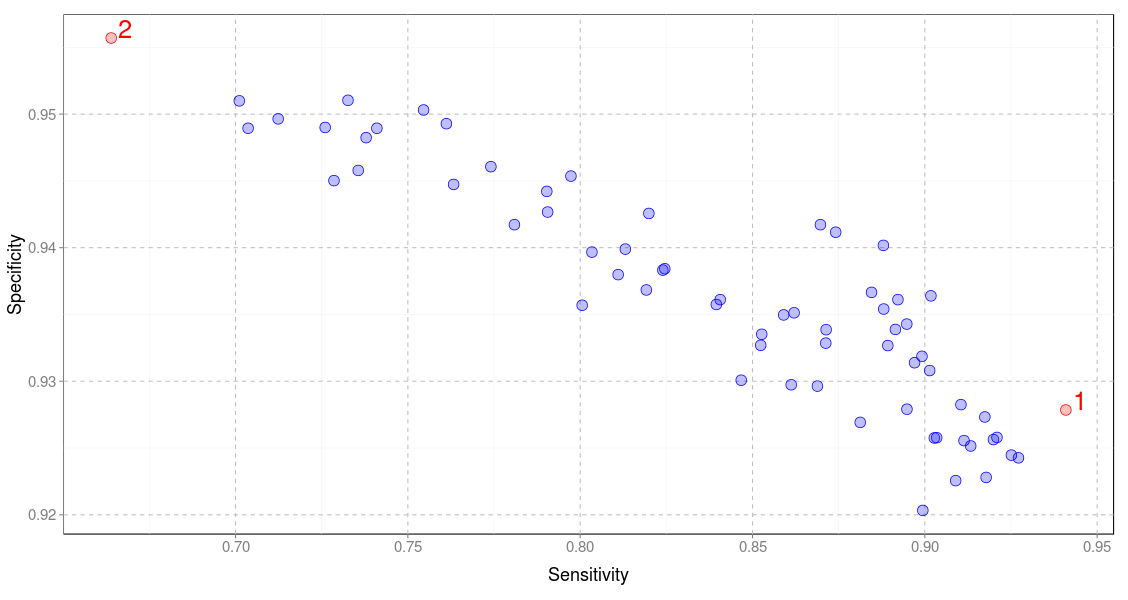
\includegraphics[width=0.9\textwidth]{figures/cvres.png}
\caption{Results of cross-validation. 1. An encoding providing the best sensitivity (AUC = 0.9687, MCC = 0.8689). 2. An encoding providing the best specificity (AUC = 0.9346, MCC = 0.6479).}
\label{fig:cvres}
\end{figure}

We used four performance measures to evaluate results of cross-validation: specificity, sensitivity, Matthew's Correlation Coefficient ($\phi$ coefficient) and Area Under the Curve (AUC). All encodings provide very good AUC (0.93 -- 0.97) and specificity (0.92 -- 0.96). The encodings have the biggest impact on sensitivity, which ranges from 0.66 to 0.94. The final signalHsmm algorithm uses the encoding, that yields the highest specificity and Matthew's Correlation coefficient as well as the second best AUC (see Fig.~\ref{fig:cvres}).

\begin{table}[ht]
\begin{minipage}{.5\linewidth} 
\centering
\begin{tabular}{l}
  \toprule
Groups \\ 
  \midrule
A, E, K, Q, R \\ 
   \rowcolor[gray]{0.85}D, G, N, P, S, T \\ 
  C, H, I, L, M, V \\ 
   \rowcolor[gray]{0.85}F, W, Y \\ 
   \bottomrule
\end{tabular}
\caption{Best-sensitivity (final) encoding.} 
\label{tab:best}
\end{minipage}
\begin{minipage}{.5\linewidth} 
\centering
\begin{tabular}{l}
  \toprule
Groups \\ 
  \midrule
D, E, H, K, N, Q, R \\ 
   \rowcolor[gray]{0.85}G, P, S, T, Y \\ 
  F, I, L, M, V, W \\ 
   \rowcolor[gray]{0.85}A, C \\ 
   \bottomrule
\end{tabular}
\caption{Worst-sensitivity encoding.} 
\label{tab:worst}
\end{minipage}
\end{table}


\begin{figure}[ht]\centering
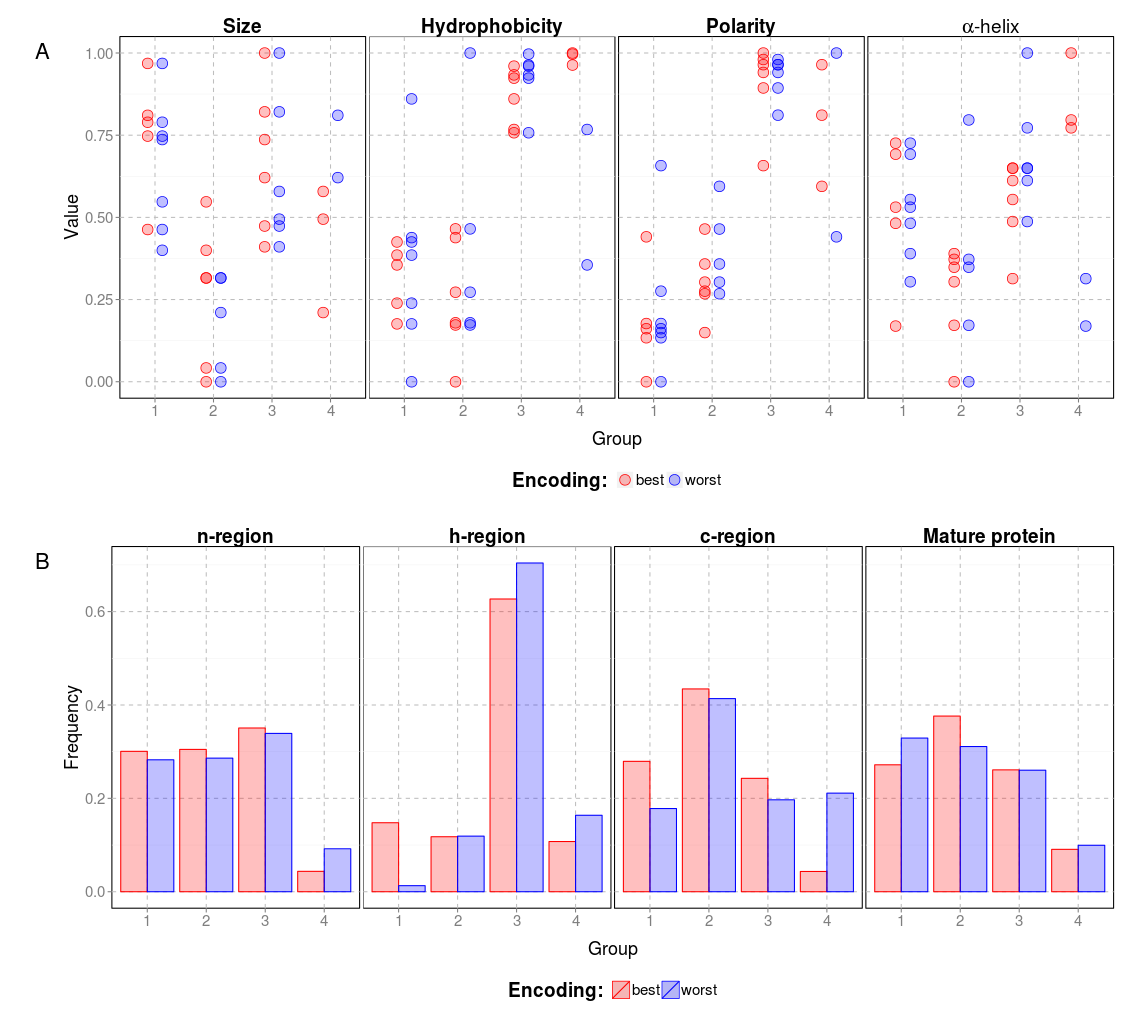
\includegraphics[width=0.9\textwidth]{figures/enccomp.png}
\caption{A comparision of encodings.}
\label{fig:enccomp}
\end{figure}

\section*{Discussion}

Despite the presence of signal peptide predicting software, there are no exhaustive studies devoted to the analysis of the signal peptide structure and taxonomical variability. Our research focuses on a transparent model of signal peptide instead of a ‘black-box’ solution.

The proposed algorithm recognizing various signal peptides will reduce costs and speed up searching appropriate artificial signal peptides designed for protein secretion in expensive and time-consuming laboratory experiments. Moreover, the algorithm can be applied in recognition any sequence types on the nucleotide and amino acid levels, represented by small sets. Accessible as a stand-alone and browser-based software, its useful both for researches interested in the analysis of signal peptides.


\section*{Acknowledgments}
PS and PB devised the HSMM model of signal peptide. MB and PS co-wrote the software. MB gathered data and carried the analysis.
MB, PS and PM drafted the manuscript. All authors revised the manuscript and approved the final version.


\bibliography{lokalizom}

\end{document}
